% http://www.ctan.org/tex-archive/macros/latex/contrib/beamer/examples
% http://latex.artikel-namsu.de/english/beamer-examples.html

\documentclass{beamer}
\usepackage{amsmath}
\usepackage{amssymb}
\usepackage{bm}
\usepackage{fancybox, graphicx}
\usepackage{listings}


\lstdefinestyle{customc}{
  belowcaptionskip=1\baselineskip,
  breaklines=true,
  %frame=L,
  xleftmargin=\parindent,
  language=bash,
  showstringspaces=false,
  basicstyle=\footnotesize\ttfamily,
  keywordstyle=\bfseries\color{green!40!black},
  commentstyle=\itshape\color{purple!40!black},
  identifierstyle=\color{blue},
  stringstyle=\color{orange},
}

\lstset{style=customc}

\usetheme{Warsaw}


\title[Linux HPC Workshop] % (optional, use only with long paper titles)
{Linux HPC Workshop}

\author[Balan,Rollins,Owen] % (optional, use only with lots of authors)
{S.~T.~Balan,\\[3mm]
R.~Rollins,~P.~Owen}

\institute[UCL]
{
  Department of Physics and Astronomy\\
  University College London
}
\date[Linux HPC 2014]
{October 2014}

\subject{Liunx and HPC}

\begin{document}

\frame{\titlepage}

\section{Basics}

\begin{frame}{How to access training materials?}
  \begin{block}{url}
    \url{https://github.com/Astrophysics-UCL/HPCInfo/tree/master/training/linux_hpc_workshop_oct_2014}
  \end{block}
\end{frame}


\begin{frame}{What will you learn?}
  \begin{itemize}
    \item Accessing Astrophysics group machines
    \item Using linux console for your research
    \item Running your programs in HPC machines
  \end{itemize}
\end{frame}

\begin{frame}[fragile]{Accessing machines from outside}
  \alert{You will need a \emph{username} and \emph{password}}
  \begin{block}{steps}
    \lstinputlisting{commands/login.sh}
  \end{block}
\end{frame}

\begin{frame}[fragile]{command structure}
  \begin{block}{structure}
    \lstinputlisting{commands/command.sh}
  \end{block}
  \begin{example}
    \lstinputlisting{commands/command_example.sh}
  \end{example}
\end{frame}


\begin{frame}[fragile]{Linux console cheat sheat I}
  \fontsize{7pt}{7}\selectfont
  \begin{columns}
    \column{.5\textwidth}
    \begin{block}{navigation and help}
      \lstinputlisting{commands/navigation.sh}
    \end{block}
    \begin{block}{copy or move}
      \lstinputlisting{commands/copy_move.sh}
    \end{block}

    \column{.5\textwidth}
    \begin{block}{create or delete}
      \lstinputlisting{commands/make_delete.sh}
    \end{block}
    \begin{block}{find or search}
      \lstinputlisting{commands/find_search.sh}
    \end{block}
  \end{columns}
\end{frame}

\begin{frame}[fragile]{Linux console cheat sheat II}
  \fontsize{7pt}{7}\selectfont
  \begin{columns}
    \column{.5\textwidth}
    \begin{block}{file contents}
      \lstinputlisting{commands/file_contents.sh}
    \end{block}
    \begin{block}{process management}
      \lstinputlisting{commands/process_management.sh}
    \end{block}

    \column{.5\textwidth}
    \begin{block}{ssh}
      \lstinputlisting[language=bash]{commands/ssh_scp.sh}
    \end{block}
    \begin{block}{system info}
      \lstinputlisting[language=bash]{commands/system_info.sh}
    \end{block}
  \end{columns}
\end{frame}


\begin{frame}[fragile]{Linux console cheat sheat III}
  \fontsize{7pt}{7}\selectfont
  \begin{columns}
    \column{.5\textwidth}
    \begin{block}{\& ; $|$ > <}
      \lstinputlisting[language=bash]{commands/wild_card.sh}
    \end{block}
    \begin{block}{Text editors}
      \lstinputlisting[language=bash]{commands/text_editors.sh}
    \end{block}

    \column{.5\textwidth}
    \begin{block}{web}
      \lstinputlisting[language=bash]{commands/web.sh}
    \end{block}
    \begin{block}{publishing}
      \lstinputlisting[language=bash]{commands/publishing.sh}
    \end{block}
  \end{columns}
\end{frame}

\begin{frame}[fragile]{Linux console cheat sheat IV}
  \fontsize{7pt}{7}\selectfont
  \begin{columns}
    \column{.5\textwidth}
    \begin{block}{compressed files}
      \lstinputlisting[language=bash]{commands/compress.sh}
    \end{block}
    \begin{block}{images}
      \lstinputlisting[language=bash]{commands/images.sh}
    \end{block}

    \column{.5\textwidth}
    \begin{block}{development}
      \lstinputlisting{commands/development.sh}
    \end{block}
    \begin{block}{scientific}
      \lstinputlisting{commands/scientific.sh}
    \end{block}
  \end{columns}
\end{frame}

\begin{frame}{Exercises I}
  \fontsize{8pt}{8}\selectfont
  \begin{enumerate}
    \item In your home directory create a dirctory called \texttt{linux\_hpc\_workshop}
    \item Change directory to \texttt{linux\_hpc\_workshop}
    \item What is the present working directory
    \item Make a directory \texttt{level\_1/level\_2}, and move to \texttt{level\_1/level\_2} in one command
    \item Move back to previous directory
    \item Remove the directory (and its contents) \texttt{level\_1}
    \item Make a symbolic link to \texttt{usr/lib} in the current directory called \texttt{my\_sybolic\_link}
    \item Create a file called \texttt{bla.txt} contents ``this file has a word called bla''
    \item Add another line in \texttt{bla.txt} called ``this is the second line''
    \item Check if it worked
    \item Search for the phrase \emph{bla} in \texttt{bla.txt}
  \end{enumerate}
\end{frame}


\begin{frame}{Exercises II}
  \fontsize{8pt}{8}\selectfont
  \begin{enumerate}
    \item Find the location of your python installation
    \item Find the installtion location(s) of \texttt{liblapack.a}
    \item Find whether an object \texttt{daxpy} is in \texttt{liblapack.a}
    \item Find the value the environment variable \texttt{PATH} and \texttt{LD\_LIBRARY\_PATH}
    \item Set the environment variable \texttt{MY\_LINUX\_HPC\_VAR} to the absolute path to \texttt{linux\_hpc\_workshop}
    \item Add, i.e append the absolute path to \texttt{linux\_hpc\_workshop} to the \texttt{PATH}
    \item Use the source command do the last two steps from source file.
    \item Use man command to find the option of \texttt{ls} that shows the output in Kilobyte,Megabyte
  \end{enumerate}
\end{frame}

\begin{frame}{Exercises III}
  \fontsize{8pt}{8}\selectfont
  \begin{enumerate}
    \item Find hostname,processor type,operating system version and write these info inot a text file called \texttt{info.txt}
    \item Find the list of people who are loged into the system
    \item Find the process that is taking most of the CPU at the moment
    \item Find ids of the processes that you are running
    \item Make a directory called \texttt{to\_be\_compressed}. Add the files \texttt{hello.cpp} and \texttt{hello.py} in this dir
    Now compress this directory using tar and zip
    \item Delete the dirctory \texttt{to\_be\_compressed} and extract the files from \texttt{to\_be\_compressed.tar.gz}
    \item Use wget to download  files from \url{ftp://heasarc.gsfc.nasa.gov/software/fitsio/c/cfitsio3370.tar.gz}
    \item What is the size of the item you just downloaded in MB
    \item Find the number of occurrences of the phrase \texttt{table} is easy in all the files with extension \texttt{.h}
    \item Remove all the fiels with extension \texttt{.h}
    \item Copy the files with extension \texttt{.c} into a new directory \texttt{c\_files}
  \end{enumerate}
\end{frame}

\begin{frame}{HPC Facilities}
  \begin{table}
    \begin{tabular}{|c|c|c|c|}
      \hline
      machine & type & cores & memory  \\
      \hline
      \textsc{splinter}-1 & distributed & 96 & 48GB  \\
      \textsc{splinter}-2 & shared & 40 & 1TB \\
      \textsc{phalanx} & shared & 32 & 512GB \\
      \hline
    \end{tabular}
  \end{table}
\end{frame}

\begin{frame}{\textsc{splinter} distributed}
  \begin{figure}
    \begin{center}
      \shadowbox{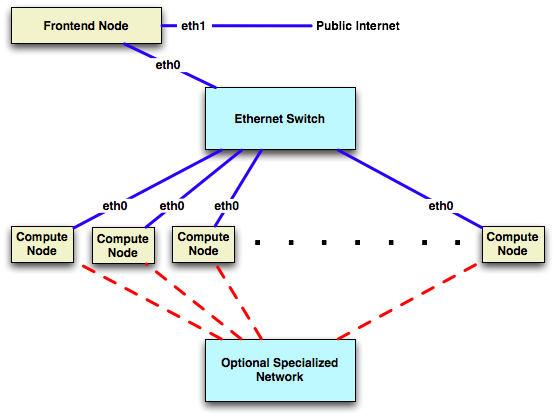
\includegraphics[scale=0.4]{img/cluster.png}}
      \footnote{\url{http://www.rocksclusters.org/}}
    \end{center}
  \end{figure}
\end{frame}

\begin{frame}{\textsc{splinter} shared}
  \begin{figure}
    \begin{center}
      \shadowbox{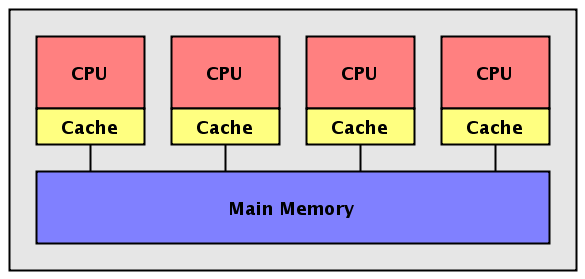
\includegraphics[scale=0.4]{img/fig03.png}}
      \footnote{\url{http://www.cs.rit.edu/}}
    \end{center}
  \end{figure}
\end{frame}

\begin{frame}{Best practices I}
  \begin{itemize}
    \item Choose the machines that are suited for your problem
    \item Read the User Guide
    \item Do not run your programs in the login node
    \item Do not install common software locally
    \item Request optimum resouces
    \item Minimise data transfer between nodes,
    \item \alert{Backup! Backup! Backup!}
  \end{itemize}
\end{frame}

\begin{frame}[fragile]{Submitting jobs}
  \fontsize{9pt}{9}\selectfont
  \begin{columns}
    \column{.3\textwidth}
    \begin{block}{commands}
      \lstinputlisting{commands/job_submission.sh}
    \end{block}

    \column{0.7\textwidth}
    \begin{example}
      \lstinputlisting{commands/sample_job_script.sh}
    \end{example}
  \end{columns}
\end{frame}

\begin{frame}{Exercises III}
  \fontsize{10pt}{8}\selectfont
  \begin{enumerate}
    \item Login to your HCP machine and find the path to your \texttt{HOME}
    directory and your quota
    \item Find the processor type and the version of your operating system
    \item Request an interative \texttt{queue} and run the \texttt{hello\_world.exe}
    \item Sumbit \texttt{hello\_world.exe} using a job script, find its \texttt{jobid}, check the output log.
    \item Compile \texttt{big\_mem\_example}, submit it using a \texttt{job-script} and see how much menory it uses
    \item Compile \texttt{time\_pause\_example}, submit it using a \texttt{job-script} and kill this job using its \texttt{jobid}.
    \item In the previous example see what happens when you play with the time requested.
  \end{enumerate}
\end{frame}


\begin{frame}{More information}
  \begin{block}{ap-wiki}
    \url{http://www.ucl.ac.uk/star/GroupAWiki}
  \end{block}

  \begin{block}{UCL Research Computing Platforms}
    \url{https://wiki.rc.ucl.ac.uk/wiki/Main_Page}
  \end{block}

  \begin{block}{DiRAC}
    \url{http://www.dirac.ac.uk/}
  \end{block}
\end{frame}


\end{document}
